\section{Introduction}
\label{sec:introduction}

Imaging systems rarely observe an image directly: MRI chooses k-space
trajectories, CT chooses projection angles, and programmable LiDAR chooses
angular cells.  When time, dose, or bandwidth is scarce,
the next measurement should depend on what remains uncertain for the current
subject.  Diffusion inverse solvers make this appealing
\cite{song2023pigdm,chung2023dps}: they can turn a severely
undersampled measurement into a rich conditional distribution rather than a
single reconstruction.  Yet a useful active policy must compress that
distribution, compare thousands of physically grouped actions, imagine
possible outcomes, and update the reconstruction before the next acquisition.

Diffusion acquisition methods expose a trade-off.
Particle methods use several posterior trajectories to rank measurements
\cite{nolan2025ads,elata2024adasense,morssy2024informed}.  They retain
multimodality, but endpoint disagreement is expensive and contains no
within-trajectory uncertainty.  Local Tweedie/Jacobian methods extract
posterior second moments from a denoiser
\cite{manor2024posterior,rissanen2025freehunch,schioppa2026covariance}; however,
one covariance replaces an ambiguous posterior with one Gaussian.  For a
frozen linear Gaussian belief, conditional covariance is outcome-independent,
so information planning has no advantage over open loop: the representation
removes the phenomenon adaptivity should exploit.

We ask whether a few diffusion branches and local tangent directions can
complement one another.  At an
acquisition checkpoint, branch $k$ provides a clean mean $m_k$ and a
rank-$r_k$ factor $U_k$ obtained from denoiser Jacobian-vector products.  The
resulting belief
\begin{equation}
    \widehat p(x\mid y_M)
    =\sum_{k=1}^{K} w_k\,
      \N(x;m_k,U_kU_k^\top)
    \label{eq:intro-mixture}
\end{equation}
Rao--Blackwellizes uncertainty: branch means retain global ambiguity, while
local factors integrate within-branch variation analytically.  The method
contains a particle belief when $r_k=0$ and a one-state covariance method when
$K=1$, making both failure modes explicit ablations.

Naively, a Gaussian mixture does not solve the scaling problem.  One
multicoil phase-encode line may contain tens of thousands of real scalar
measurements, and non-myopic planning appears to require repeated high
dimensional likelihoods.  Our central observation is that action $a$ depends
on the belief only through the whitened span of its pushed local factors and
branch-mean offsets.  Its dimension is at most
\begin{equation}
    d_a\leq \sum_{k=1}^K r_k + K-1,
    \label{eq:intro-rank}
\end{equation}
regardless of the number of coils, readout samples, pixels, or angular cells in the
action.  Projected fantasy observations are sufficient for component
likelihoods and exact Gaussian conditioning under the surrogate.  A
horizon-two tree therefore adds matrix and mixture operations but no denoiser
evaluation.  Figure~\ref{fig:overview} summarizes the loop.

\begin{figure*}[t]
    \centering
    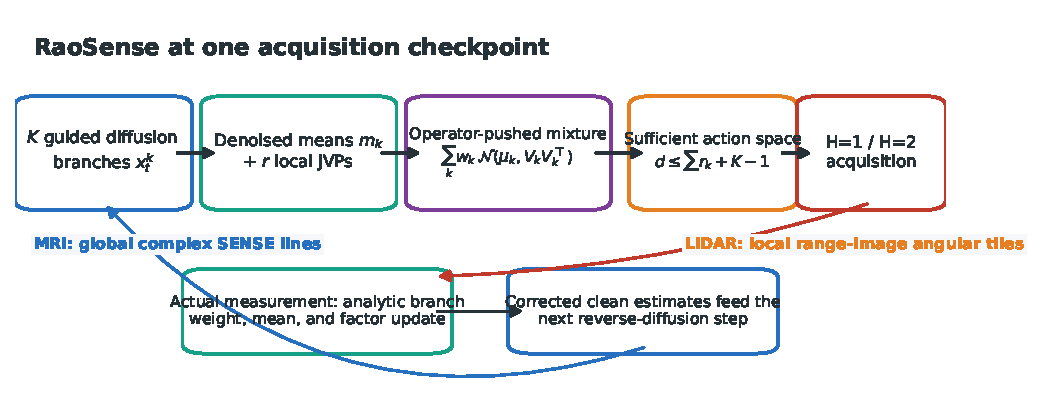
\includegraphics[width=\textwidth]{figures/method_overview.pdf}
    \caption{\textbf{\method{} loop.} A few measurement-guided reverse
    trajectories retain between-mode ambiguity; local denoiser JVPs retain
    within-mode uncertainty.  Both are pushed through the feasible operator
    bank.  Information scoring, fantasy planning, and the actual Bayesian
    update occur in a small sufficient space.  Only the real measurement is
    executed, after which corrected branch means continue through diffusion.
    The same algebra selects global complex SENSE lines and local LiDAR angular
    tiles.}
    \label{fig:overview}
\end{figure*}

The second obstacle is operator uncertainty.  Active diffusion work almost
universally assumes that the forward model is known, while blind diffusion
reconstruction estimates an operator under a fixed measurement set
\cite{chung2023blinddps,chen2025jsmoco}.  Treating uncertain coil maps, motion,
or beam geometry as known overstates how informative an action is about the
image.  We augment each local branch with a gauge-fixed nuisance factor and
derive information about the target image while marginalizing nuisance.  The
result separates measurements that resolve anatomy from measurements whose
apparent utility merely relies on perfect calibration.

The contribution is not ``Gaussian mixtures for sensing,'' ``mutual
information,'' or ``non-myopic planning'' in isolation; all are classical
\cite{braun2015infogreedy,huan2016soed,guo2026copex}.  Our claim is the
diffusion-derived \emph{operator-sufficient belief} that makes their useful
combination tractable at imaging scale.  Specifically:
\begin{itemize}
    \item We combine between-trajectory modes with within-trajectory
    Tweedie/JVP factors and preserve the mixture through acquisition and
    reconstruction updates.
    \item We derive an exact within/mode information decomposition, a lower
    and two-way upper information sandwich, safe one-step pruning, and the
    sufficient dimension bound in Eq.~\eqref{eq:intro-rank}.
    \item We implement receding-horizon outcome planning and analytic branch
    correction with no fantasy denoiser calls.  We explicitly characterize
    beam and candidate truncation as approximations, not certified pruning.
    \item We extend the objective to joint image/operator beliefs and
    preregister a two-domain evaluation on pathology-annotated raw multicoil
    MRI and programmable LiDAR, with matched NFE, prior-specific replay, and
    patient/drive-level inference.
\end{itemize}

The current synthetic results validate algebra and falsification machinery,
not imaging quality.  We retain visible placeholders rather than convert
legacy frequency-domain experiments into evidence for a different method.
